

\documentclass[11pt]{amsbook}

\usepackage{../HBSuerDemir}	% ------------------------


\begin{document}

% ++++++++++++++++++++++++++++++++++++++
\hPage{b2p2/312}
% ++++++++++++++++++++++++++++++++++++++
\begin{align*}
4A \frac{\hDif A}{\hDif t} = x(y^2+z^2) \frac{\hDif x}{\hDif t} + y(z^2+x^2) \frac{\hDif y}{\hDif t} + z(x^2+y^2)  \frac{\hDif z}{\hDif t}
\end{align*}

When P is at $P_{O}$(6, 0, 0), then Q is at $Q_{O}$(0, 9, 0) and R is at $R_{O}$(0, 0, 12) with $|P_{O}$  $Q_{O}$  $R_{O}|_{2}$ = 9$\sqrt{61}$. Then

\begin{align*}
4.9\sqrt{61}\frac{\hDif A}{\hDif t} = 6(225)2+ 9(680)3 + 12(117)4 \\
9\sqrt{61}\frac{\hDif A}{\hDif t} = 675 + 27.45 + 12.117 \\
\sqrt{61}\frac{\hDif A}{\hDif t} = 75 + 135 + 156 = 366 \\
\frac{\hDif A}{\hDif t} = \frac{766}{\sqrt{61}} = 6\sqrt{61}  unit^2/sec
\end{align*}

\subsection{TAYLOR'S FORMULA AND SERIES}

\begin{thm} If f(x, y) has continuous partial derivatives up to order n+1 in a neighborhood of (a, b)$\epsilon \upsilon_{f}$, then
\begin{align*}
f(x, y) = f(a, b) +  \sum_{k=1}^{n}  \frac{1}{k!} ((x-a) \frac{a}{ax} + (y-b) \frac{a}{ay})^k f(x, y) |_{(a, b)} + R_{n+1}
\end{align*}
where the remainder is given by
\begin{align*}
R_{n+1} = \frac{1}{(n+1)!} ((x-a) \frac{a}{ax} + (y-b) \frac{a}{ax})^{n+1}f(x, y)_{(x*, y*)}
\end{align*}
with (x*, y*) a point on the open segment ($P_{O}$P) joining $P_{O}$(a, b) to P(x, y) 
\end{thm}
\begin{proof} Since every point of the line segment [$P_{O}$P] can be represented parametrically as



\begin{align*}
x = a+ht,\qquad   y = b+kt\qquad	  0\leq t \leq 1,
\end{align*} 

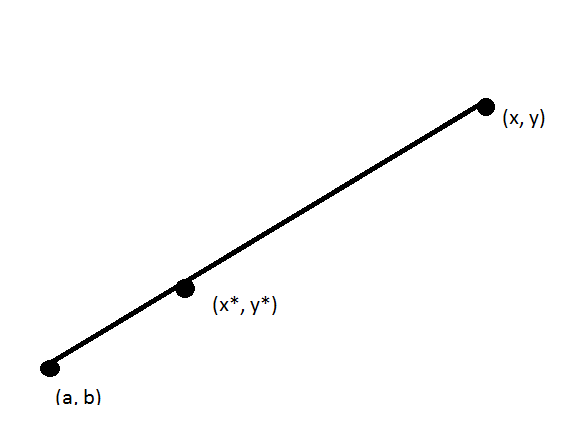
\includegraphics[width=0.35\textwidth]{images/b2p2-312-fig01}

The end points of the segment correspond to t=0 and t=1 (observe that h, k are direction numbers of the line segment)
Substituting (2) in f(x, y) gives the function

\end{proof}


\end{document}  